\documentclass[a4paper,10.5pt]{report}

\usepackage[toc]{appendix}
\usepackage[catalan]{babel}
\usepackage{tcolorbox}
\usepackage{parskip}
\usepackage{multirow}
\usepackage{graphicx}
\usepackage{booktabs}
\usepackage{caption}
\captionsetup{labelfont=bf}
\usepackage{hyperref}
\usepackage[arrowdel]{physics}
\usepackage[left=1.95cm, right=1.95cm, top=20mm, bottom=20mm]{geometry} 
\usepackage{fancyhdr}
\usepackage{braket}
\usepackage{amssymb}
\usepackage{subcaption}
\usepackage{cancel}
\usepackage{float}
\usepackage{titling}
\usepackage{etoolbox}

%Definim el següent entorn per tal de poder posar abstracts a cada capítol.
\newenvironment{chapterabstract}{
	\begin{center}
		\bfseries Abstract
	\end{center}
	\quotation
}{\endquotation}

\usepackage{titlesec}
\usepackage{tikz}


\titleformat{\chapter}[display]{\normalfont\huge\bfseries}{Pràctica \thechapter}{0pt}{\vspace{0.2cm}\huge\bfseries\raggedright}

\title{\textbf{\huge{Informes de Pràctiques. \\ \vspace{0.2cm} Laboratori d'Electromagnetisme}}}
\author{Grup A1}
\date{\today}

\begin{document}
	
\begin{titlepage}
	\centering
	{\LARGE Laboratori d'Electromagnetisme \par}
	\vspace{2cm}
	{\Huge \textbf{Informes de Pràctiques} \par}
	\vspace{3cm}
	{\Large Grup A1 \par}
	\vspace{0.5cm}
	{\Large 1549086: Bujones Umbert, Jun Shan\\1669619: Rama Ariza, Raul\\  1672980: González Barea, Eric\\1644841: Vilarrúbias Morral, Natàlia \par}
	\vspace{2cm}
	{\Large Març $-$ Maig 2025 \par}
	\vspace{2cm}
	
	\begin{figure}[h]
		\centering
		
\includegraphics[width=0.3\linewidth]{screenshot001}
		\label{fig:screenshot001}
	\end{figure}
\end{titlepage}

\tableofcontents
\newpage

\chapter{Representació de camps} 

\begin{chapterabstract}
	En aquesta pràctica estudiem diferents problemes electrostàtics en medis conductors aprofitant la dualitat existent entre la densitat de corrent $\vec{J}$ i el vector desplaçament $\vec{D}$. El nostre objectiu és trobar experimentalment les superfícies equipotencials per a determinades geometries, amb una simetria tal que podem reduir el problema a dues dimensions espacials. Una de les distribucions de càrrega amb què treballem és un condensador de plaques planoparal·leles ideal; per aquest cas, a més a més, fem el càlcul de la seva capacitat per unitat de longitud, partint del teorema de Gauss.
\end{chapterabstract}

\section{Introducció i fonament teòric}
Per a materials lineals, isòtrops i homogenis, sota la presència d'un camp electrostàtic $\vec{E}$ s'apliquen les següents equacions si el medi és conductor:
\begin{align}
	\vec{\nabla} \cross \vec{E} = 0 \\
	\vec{J} = \sigma \vec{E} \label{eq1.2}  \\ 
	\vec{\nabla}\cdot \vec{J} = 0 \label{eq1.3}
\end{align}
O, si el medi és dielèctric:
\begin{align}
	\vec{\nabla} \cross \vec{E} = 0 \\
	\vec{D} = \varepsilon \vec{E} \label{eq1.5} \\ 
	\vec{\nabla}\cdot \vec{D} = 0 \label{eq1.6}
\end{align}

Per aquest tipus de medis $\varepsilon$ i $\sigma$ són constants, així, combinant les darreres equacions trobem:
\begin{align}
	\vec{\nabla} \cross \vec{J} = 0 \\
	\vec{\nabla} \cross \vec{D} = 0
\end{align}
Això últim implica que tant $\vec{J}$ com $\vec{D}$ són camps conservatius i, per tant, es poden definir com el gradient (canviat de signe) d'una funció escalar, és a dir:
\begin{align}
	\vec{J} = -\vec{\nabla}{U} \\
	\vec{D} = -\vec{\nabla}{U'}
\end{align}
A partir de les equacions \eqref{eq1.3} i \eqref{eq1.6} podem deduir
\begin{equation}
	\nabla^2 U  = 0, \hspace{0.25cm} \nabla^2 U' = 0 \label{eq1.11}
\end{equation}
que són les corresponents equacions de Laplace. Així, donat uns potencials escalars $U$ i $U'$ que satisfacin les condicions de contorn i \eqref{eq1.11}, podem trobar $\vec{J}$ i $\vec{D}$, respectivament.

Si comparem les equacions \eqref{eq1.2} i \eqref{eq1.5} per una banda i les equacions \eqref{eq1.3} i \eqref{eq1.6}, podem veure que qualsevol solució per $\vec{J}$ és també una solució vàlida per $\vec{D}$, sempre que estiguem sota condicions de contorn equivalents i que ni $\sigma$ ni $\vec{E}$ presentin discontinuïtats. Per tant, si coneixem una solució per un medi conductor, podrem trobar-ne una equivalent pel medi dielèctric intercanviant $\varepsilon$ per $\sigma$.

Recordem que per poder calcular la capacitat per unitat de longitud d'un condensador de plaques planoparal·leles, considerem una superfície equipotencial que tanca una de les plaques del condensador. En virtut del teorema de Gauss tenim que:

\begin{equation}
	q = \varepsilon \int_S \vec{E}\cdot \vec{n}dS
\end{equation}

Assumint que el condensador és infinitament llarg en la direcció $z$, podem assegurar que el camp és constant en aquesta direcció i, per tant, $dS = Zdl$, on $dl$ és el diferencial de longitud a la intersecció de la superfície equipotencial amb un pla perpendicular al condensador \textbf{POSAR FOTO}. Amb això tenim que
\begin{equation}
	\frac{q}{Z} = \varepsilon \oint_C E dl \label{eq1.13}
\end{equation}

\section{Metodologia experimental}
\subsection{Representació de corbes equipotencials}
Per tal de poder representar les línies equipotencials usem fulls de paper impregnats amb carbó de resistències compreses en un rang de 5 k$\Omega$ $-$ 20 k$\Omega$ per quadrat, que actuaran com a medis conductors (de conductivitat $\sigma$ homogènia) entre els elèctrodes. Les distribucions de càrrega (elèctrodes) les dibuixem usant un retolador que desprèn una tinta conductora, produïda per partícules de plata en suspensió en un líquid (veure figura \ref{fig1.1a}); per assegurar-nos que la conductivitat d'aquesta tinta esdevé màxima deixem reposar durant 20 minuts, aproximadament. Per evitar possibles problemes de falta de càrregues als elèctrodes, ens hem assegurat de dibuixar línies suficientment gruixudes.

\begin{figure}[h]
	\centering
	\begin{subfigure}{0.45\textwidth}
		\centering
		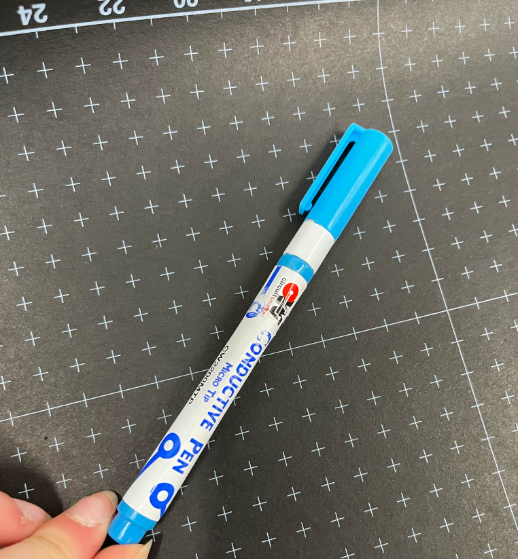
\includegraphics[width=\linewidth]{screenshot002}
		\caption{Paper conductor i retolador de tinta basada en una suspensió de plata.}
		\label{fig1.1a}
	\end{subfigure}
	\hfill
	\begin{subfigure}{0.45\textwidth}
		\centering
		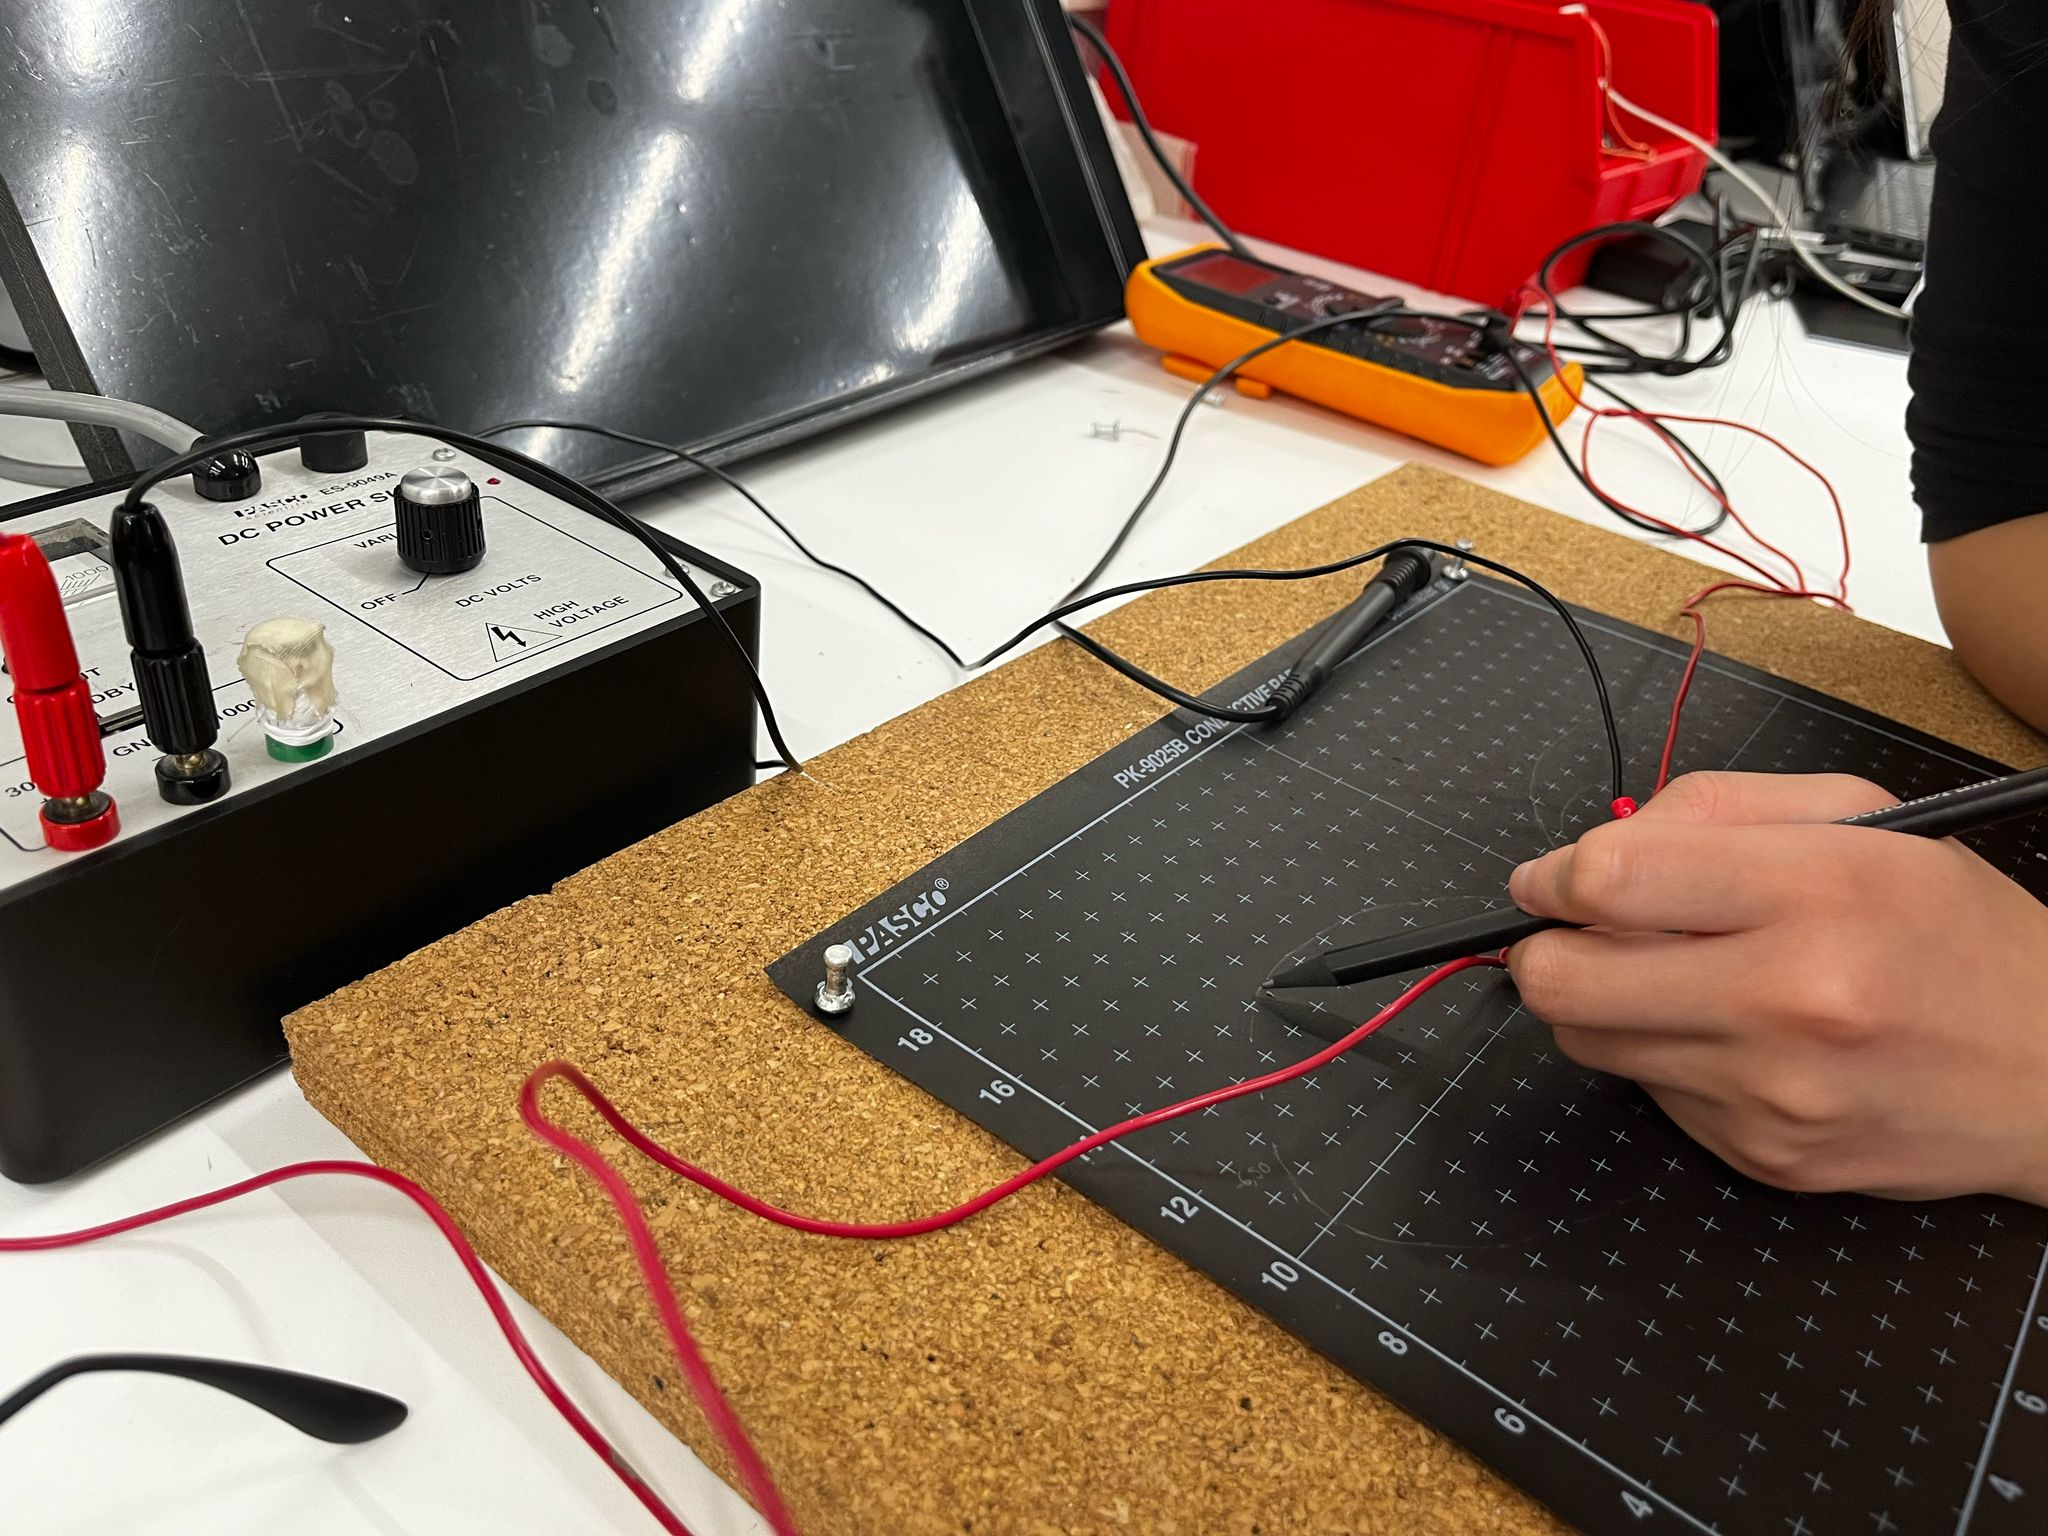
\includegraphics[width=\linewidth]{screenshot003}
		\caption{Muntatge experimental per a la representació de les corbes equipotencials pels dos fils infinits. D'esquerra a dreta: Font de corrent DC connectada als dos elèctrodes (dos punts pel cas representat) mitjançant dos cables; suro amb el paper conductor en el que prèviament s'han dibuixat els dos elèctrodes, enganxat amb xinxetes; multímetre usat per mesurar les diferències de potencial.}
		\label{fig1.1b}
	\end{subfigure}
	\caption{Paper conductor i muntatge experimental per a la representació de les corbes equipotencials.}
	\label{fig1.1}
\end{figure}



Hem treballat amb les següents 3 distribucions: dues línies verticals (que són la projecció d'un condensador de plaques planoparal·leles), dos punts (projecció de dos fils infinits) i dues línies secants amb un punt entre elles (projecció de dos plans infinits formant angle d'aproximadament 60 º amb un fil infinit entre els dos).

Amb el pretext de generar el camp sobre les distribucions dibuixades, s'ha fixat el paper conductor (en el qual hem fet els dibuixos) sobre un suro usant xinxetes i hem connectat els elèctrodes (per a cada distribució per separat) a una font de corrent continu (DC) usant un parell de cables i més xinxetes. Per mesurar la diferència de potencial hem usat un multímetre, deixant un cable fixat a un dels dos elèctrodes (establint així una referència de potencial) i l'altre lliure per tal de fer mesures de $\Delta V$ a qualsevol altre punt del paper (veure figura \ref{fig1.1b}). Prèviament, però, ens hem assegurat què la diferència de potencial entre dos punts en els conductors (els elèctrodes dibuixats) no fos major de l'1\%\footnote{Recordem que, per ser aquests materials conductors, hem de tenir un potencial constant en tot el seu volum i, en particular, sobre la seva superfície.}.

Per dibuixar les corbes equipotencials usem el cable lliure del multímetre per buscar aquestes corbes sobre el paper. Marquem tots els punts que estan a un mateix potencial amb un llapis i, tot seguit, unim aquests punts amb una línia. Repetint això un seguit de cops podem construir vàries corbes equipotencials. Per tal d'assegurar-nos que es tanquen, és millor que comencem a buscar les corbes des de l'exterior dels nostres elèctrodes. Si comencem per l'interior, com que tindrem una densitat de corbes molt major, serà més fàcil que la línia escollida no s'acabi tancant. Veurem que ens interessa trobar corbes que tanquin els nostre elèctrodes per tal de poder aplicar el teorema de Gauss (en especial pel cas del condensador de plaques planoparal·leles).

Finalment, per representar el camp elèctric $\vec{E}$, hem dibuixat línies que sortien dels elèctrodes i tallaven les corbes equipotencials perpendicularment (en ambdós casos). 

\subsection{Càlcul de la capacitat del condensador}
Si aproximem la integral donada per l'equació \eqref{eq1.13} per un sumatori i calculem el camp $E_i$ segons
\begin{equation}
	E_i \approx \frac{\Delta V_i}{\Delta r_i}
\end{equation}
on $\Delta r_i$ és la distància radial i $\Delta V_i$ és la diferència de potencial de l'element $\Delta l_i$ tenim:
\begin{equation}
	\frac{q}{Z} \approx \varepsilon \sum_i \frac{\Delta V_i \Delta l_i}{\Delta r_i}
\end{equation}
Usant que la capacitat d'un condensador de plaques planoparal·leles es correspon amb 
\begin{equation}
	c = \frac{q}{\Delta V}
\end{equation}
tenim que la capacitat per unitat de longitud, sota les aproximacions usades és:
\begin{equation}
	\frac{c}{Z} = \frac{Q/Z}{\Delta V} = \frac{\varepsilon}{\Delta V} \sum_i \frac{\Delta V_i \Delta l_i}{\Delta r_i}  
\end{equation}
on $\Delta V$ és la diferència de potencial a la que hem sotmès les dues plaques del condensador.

\subsection{Simulacions}
\section{Resultats i discussió}

\subsection{Condensador de plaques planoparal·leles}

\subsection{Fils infinits}
La segona configuració estudiada és la projecció en el pla $XY$ (pla de la imatge) de dos fils infinits separats per una distància constant. 

Les corbes equipotencials són les que es poden observar a la figura \ref{figfils}. Observem com aquestes formen el·lipses on els fils estan cada cop més descentrats conforme agafem corbes més externes. FER REFERÈNCIA A LA SIMULACIÓ.

\begin{figure}[h]
	\centering
	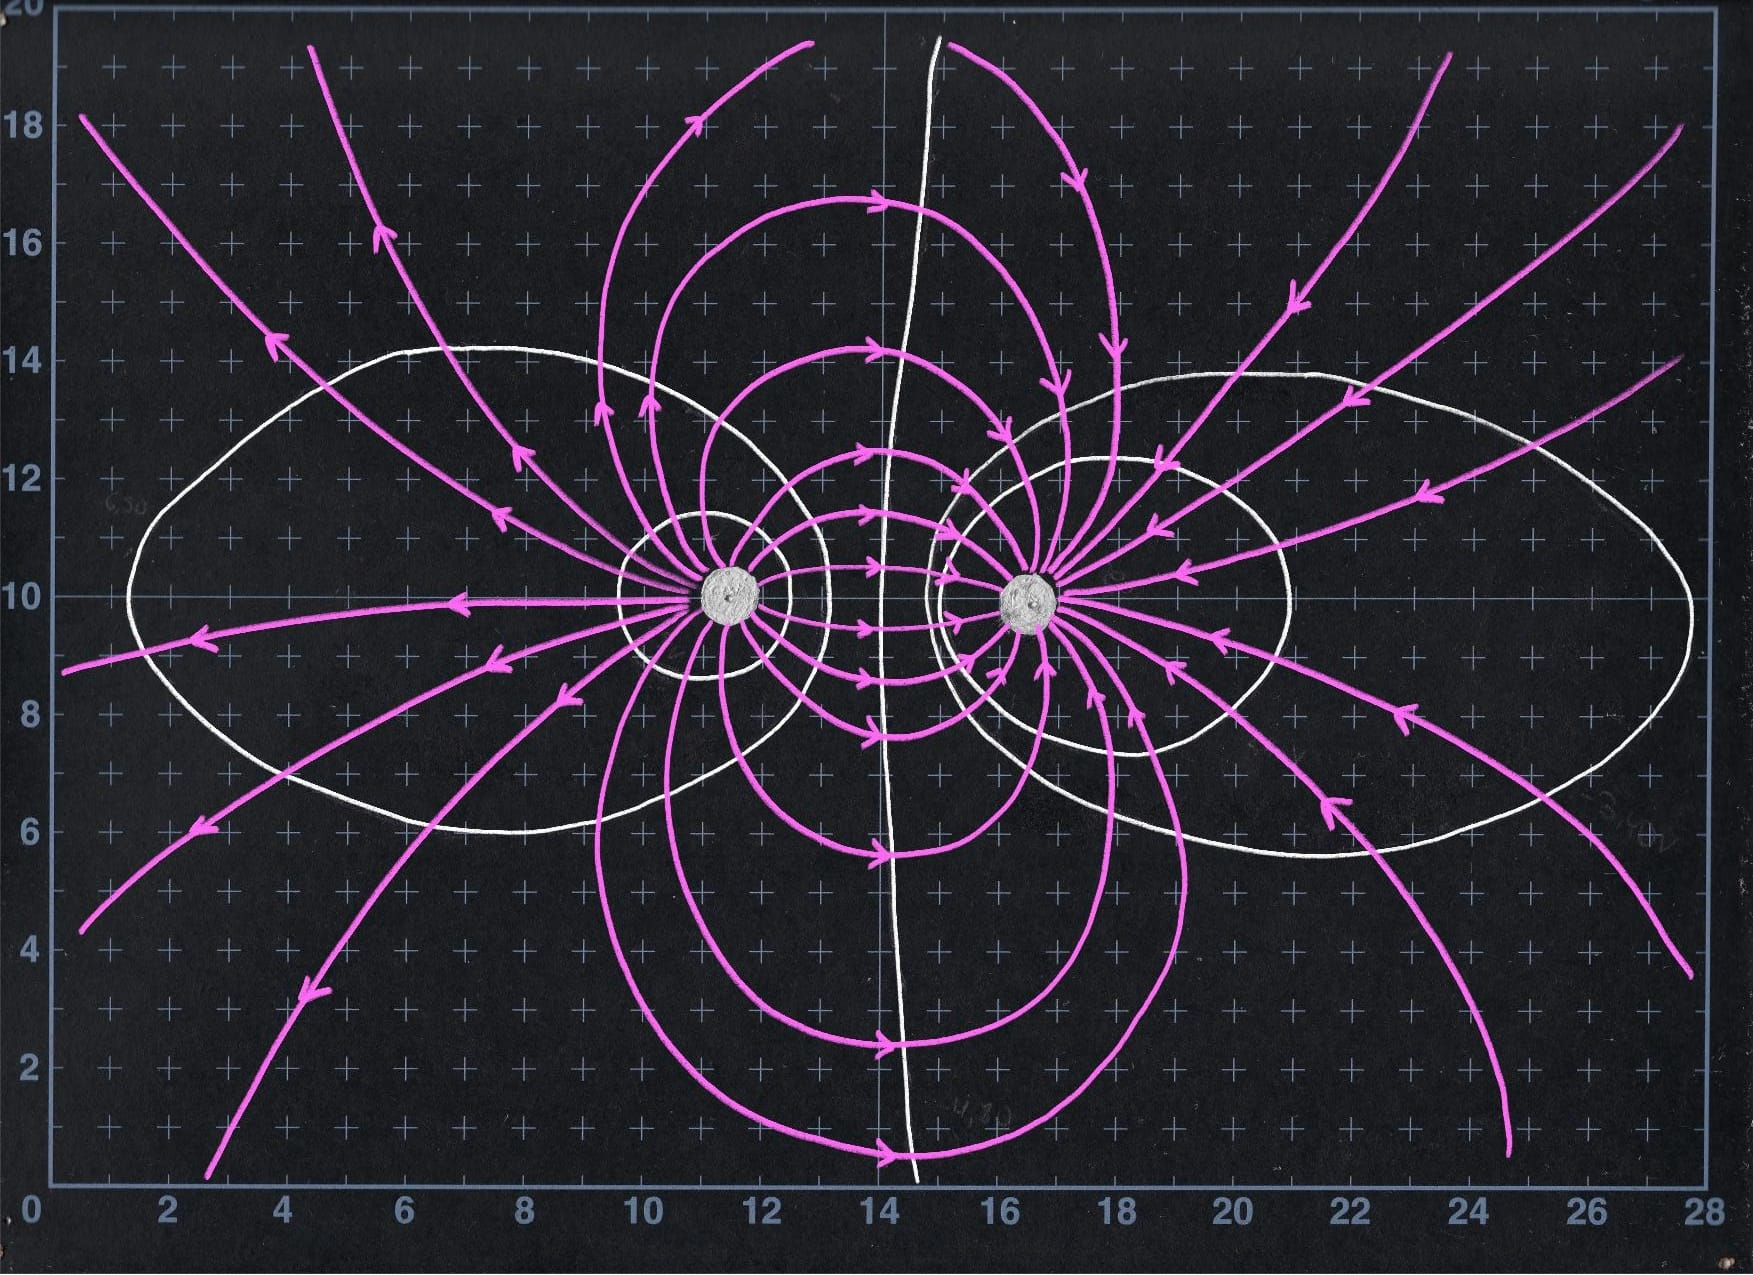
\includegraphics[width=0.5\linewidth]{screenshot004}
	\caption{Corbes equipotencials (en blanc) i línies de camp $\vec{E}$ (en lila) pel}
	\label{figfils}
\end{figure}

Els resultats teòrics indiquen que, en un sistema de dos fils infinits, les corbes equipotencials vénen donades per la següent equació:
\begin{equation}
	y^2+\left( x+a\frac{1+k^2}{1-k^2}\right)^2 = a^2\left( \frac{2k}{1-k^2}\right)^2  \label{eqsuppon}
\end{equation}
Que és l'equació d'una esfera, de manera que, teòricament, les corbes equipotencials haurien de ser circumferències de radi $R = a\frac{2k}{1-k^2}$ que tenen el seu centre lleugerament desplaçat en l'eix de les $x$ per un factor $a\frac{1+k^2}{1-k^2}$. Notem que tant $a$ com $k$ són dues constants\footnote{Aquest resultat es demostrar a l'annex ANNEX!.}. El fet que els nostres resultats es desviïn del predit per la teoria és degut als diferents errors experimentals comesos durant l'evolució de la pràctica: S'assumeix que el paper conductor té una conductivitat $\sigma$ homogènia, però això no necessàriament ha de ser així, de forma que pot alterar els resultats de l'experiment; els punts que representen la projecció dels dos fils infinits no són perfectament rodons, ja que han sigut dibuixats a ma; les corbes equipotencials i les línies de camp es poden veure afectats per l'efecte punta en les vores dels materials carregats, on s'acumula més densitat de càrrega.


\subsection{Fil infinit i dos plans}

\section{Conclusions}

\newpage
\begin{appendices}
	\textbf{\Huge{Annexos}}
	\renewcommand{\thesection}{\Alph{section}} % Cambia la numeración de capítulos a letras
	\section{Deducció de l'equació \eqref{eqsuppon}}
		
\end{appendices}


\end{document}
